\chapter{Chapter 4 --- Phase 1: Label Disagreement and Oracle
Comparison}\label{chapter-4-phase-1-label-disagreement-and-oracle-comparison}

This chapter answers \textbf{RQ1}: how much do SZZ variants disagree
with one another and with an independently constructed reference, and
what is the direction of each variant's labelling bias?

The chapter is deliberately placed before any predictive modelling.
Everything in Chapters 5 to 7 is conditioned on the noise characterised
here: the flip rates estimated in \S{}4.3 are the parameters injected in
Chapter 6, and the reference labels defined in \S{}4.1 are the scoring key
used throughout Chapter 5.

\section{4.1 Method}\label{method}

\subsection{4.1.1 The reference condition, and what it is
not}\label{the-reference-condition-and-what-it-is-not}

Every comparison in this thesis is made against \texttt{label\_oracle},
taken from JIT-Defects4J (Ni et al., ESEC/FSE 2022), itself an extension
of LLTC4J (Herbold et al.). Because the interpretation of every
subsequent result depends on exactly what these labels are, we state
their construction precisely.

The dataset authors describe a two-stage procedure. First, within each
bug-fixing commit, individual \emph{lines} were annotated as
contributing to the fix, with a line retained only where \textbf{at
least three participants assigned it the same label}. Second, for each
such verified fix line, \textbf{\texttt{git\ blame} was used to identify
the commit that introduced it}. Commits not flagged by this procedure
are treated as clean by residual.

Three consequences follow, and they constrain the claims this thesis is
entitled to make.

\textbf{The reference is not manually verified ground truth for
defect-introducing commits.} Human verification applies to the \emph{fix
lines}. The step from a fix line to an introducing commit is
algorithmic. The correct description --- used consistently throughout
this thesis --- is \textbf{\texttt{git\ blame} seeded with
human-verified fix lines}. The phrase ``developer-verified ground
truth'' is inaccurate and is not used.

\textbf{The comparison therefore isolates tangling, not total labelling
error.} SZZ blames \emph{every} line modified in a bug-fixing commit,
including refactoring, formatting and comment changes, then applies
filters to remove what it over-collected. The reference blames
\emph{only} the lines three annotators agreed were fixing the bug. Both
then apply the same blame step. What separates them is exactly one
thing: knowledge of which lines in a fix actually fix the bug. That is
the definition of a tangled commit, and it is what these comparisons
measure.

\textbf{All measured noise is consequently a lower bound.} Any
systematic error in \texttt{git\ blame} --- the syntactic line-blame
fallacy by which blame attributes a line to the last commit that touched
it rather than the one that made it wrong --- is present on \emph{both}
sides of every comparison and cancels. Noise measured against genuine
ground truth would be larger by an unknown amount.

This is a weaker claim than ``we compare SZZ against truth'', and a more
precise one. It is also the claim the data actually support.

\subsection{4.1.2 Variants, corpus and
alignment}\label{variants-corpus-and-alignment}

Six SZZ variants were executed using PySZZ v2 (Rosa et al., JSS 2023),
the reference implementation released with the developer-informed-oracle
study:

\begin{longtable}[]{@{}
  >{\raggedright\arraybackslash}p{(\linewidth - 2\tabcolsep) * \real{0.5000}}
  >{\raggedright\arraybackslash}p{(\linewidth - 2\tabcolsep) * \real{0.5000}}@{}}
\toprule\noalign{}
\begin{minipage}[b]{\linewidth}\raggedright
Variant
\end{minipage} & \begin{minipage}[b]{\linewidth}\raggedright
Refinement over its predecessor
\end{minipage} \\
\midrule\noalign{}
\endhead
\bottomrule\noalign{}
\endlastfoot
\textbf{B-SZZ} & The original: blame every line modified in the fix \\
\textbf{AG-SZZ} & Annotation-graph filtering; excludes cosmetic and
format-only changes \\
\textbf{MA-SZZ} & Additionally excludes meta-changes such as branch and
property changes \\
\textbf{R-SZZ} & Of the candidate inducing commits, retains only the
most recent \\
\textbf{L-SZZ} & Retains only the largest candidate \\
\textbf{RA-SZZ} & Refactoring-aware: removes candidates attributable to
refactorings \\
\end{longtable}

The corpus is 21 Apache Java projects, 27,319 commits, of which 2,332
(\textbf{8.54\%}) carry a reference defect label. Each variant's output
was aligned to the reference over an \textbf{identical 27,319-commit
denominator}, so that precision and recall are computed against the same
population in every row. This matters: partial denominators are a common
source of incomparability in the SZZ literature, since a variant that
emits fewer candidates can appear more precise merely by being evaluated
on a smaller set.

Per-variant quality is reported as precision, recall, F1, MCC and
Cohen's \ensuremath{\kappa}, together with the two flip rates defined in \S{}4.3.
Inter-variant agreement is reported as pairwise Cohen's \ensuremath{\kappa}.

\section{4.2 Results}\label{results}

\subsection{4.2.1 Per-variant quality against the
reference}\label{per-variant-quality-against-the-reference}

\begin{longtable}[]{@{}
  >{\raggedright\arraybackslash}p{(\linewidth - 22\tabcolsep) * \real{0.0833}}
  >{\raggedright\arraybackslash}p{(\linewidth - 22\tabcolsep) * \real{0.0833}}
  >{\raggedright\arraybackslash}p{(\linewidth - 22\tabcolsep) * \real{0.0833}}
  >{\raggedright\arraybackslash}p{(\linewidth - 22\tabcolsep) * \real{0.0833}}
  >{\raggedright\arraybackslash}p{(\linewidth - 22\tabcolsep) * \real{0.0833}}
  >{\raggedright\arraybackslash}p{(\linewidth - 22\tabcolsep) * \real{0.0833}}
  >{\raggedright\arraybackslash}p{(\linewidth - 22\tabcolsep) * \real{0.0833}}
  >{\raggedright\arraybackslash}p{(\linewidth - 22\tabcolsep) * \real{0.0833}}
  >{\raggedright\arraybackslash}p{(\linewidth - 22\tabcolsep) * \real{0.0833}}
  >{\raggedright\arraybackslash}p{(\linewidth - 22\tabcolsep) * \real{0.0833}}
  >{\raggedright\arraybackslash}p{(\linewidth - 22\tabcolsep) * \real{0.0833}}
  >{\raggedright\arraybackslash}p{(\linewidth - 22\tabcolsep) * \real{0.0833}}@{}}
\toprule\noalign{}
\begin{minipage}[b]{\linewidth}\raggedright
Variant
\end{minipage} & \begin{minipage}[b]{\linewidth}\raggedright
Precision
\end{minipage} & \begin{minipage}[b]{\linewidth}\raggedright
Recall
\end{minipage} & \begin{minipage}[b]{\linewidth}\raggedright
F1
\end{minipage} & \begin{minipage}[b]{\linewidth}\raggedright
\ensuremath{\rho}\ensuremath{_0} (false-alarm)
\end{minipage} & \begin{minipage}[b]{\linewidth}\raggedright
\ensuremath{\rho}\ensuremath{_1} (miss)
\end{minipage} & \begin{minipage}[b]{\linewidth}\raggedright
MCC
\end{minipage} & \begin{minipage}[b]{\linewidth}\raggedright
\ensuremath{\kappa}
\end{minipage} & \begin{minipage}[b]{\linewidth}\raggedright
TP
\end{minipage} & \begin{minipage}[b]{\linewidth}\raggedright
FP
\end{minipage} & \begin{minipage}[b]{\linewidth}\raggedright
FN
\end{minipage} & \begin{minipage}[b]{\linewidth}\raggedright
TN
\end{minipage} \\
\midrule\noalign{}
\endhead
\bottomrule\noalign{}
\endlastfoot
\textbf{B-SZZ} & 0.186 & \textbf{0.641} & 0.288 & 0.263 & \textbf{0.359}
& \textbf{0.232} & 0.179 & 1,495 & 6,565 & 837 & 18,422 \\
AG-SZZ & 0.186 & 0.467 & 0.266 & 0.192 & 0.533 & 0.188 & 0.163 & 1,090 &
4,786 & 1,242 & 20,201 \\
MA-SZZ & 0.183 & 0.482 & 0.265 & 0.201 & 0.518 & 0.188 & 0.161 & 1,124 &
5,030 & 1,208 & 19,957 \\
\textbf{L-SZZ} & \textbf{0.272} & 0.267 & 0.269 & \textbf{0.067} & 0.733
& 0.202 & \textbf{0.202} & 622 & 1,665 & 1,710 & 23,322 \\
R-SZZ & 0.232 & 0.300 & 0.262 & 0.093 & 0.700 & 0.185 & 0.183 & 699 &
2,316 & 1,633 & 22,671 \\
RA-SZZ & 0.184 & 0.438 & 0.259 & 0.181 & 0.562 & 0.178 & 0.158 & 1,022 &
4,531 & 1,310 & 20,456 \\
\end{longtable}

Two observations dominate.

\begin{figure}
\centering
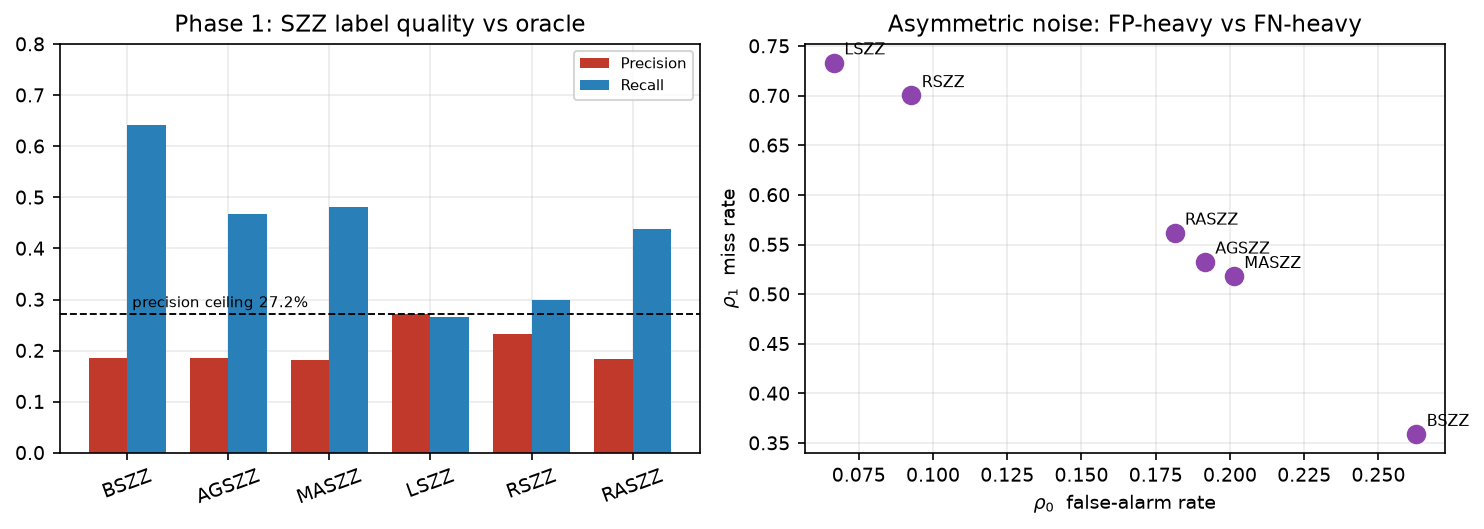
\includegraphics[width=\linewidth,keepaspectratio]{reports/figures/f1_phase1_noise.png}
\label{fig:f1_phase1_noise}
\caption{Phase 1 noise profile --- precision and recall per variant, and
the false-alarm against miss trade-off}
\end{figure}

\textbf{Figure 4.1 --- Reading the figure.} \emph{Left:} each variant's
precision (how much of what it flags is right) beside its recall (how
much of what exists it catches). The dashed line marks the 27.2\%
precision ceiling no variant exceeds. \emph{Right:} each variant plotted
by false-alarm rate \ensuremath{\rho}\ensuremath{_0} against miss rate \ensuremath{\rho}\ensuremath{_1}. \textbf{The points do not
cluster --- they spread along a diagonal}, which is the visual signature
of a trade-off rather than of random error.

\textbf{A precision ceiling at 27.2\%.} No variant exceeds it. Between
72.8\% and 81.5\% of every commit any variant flags as
defect-introducing is not one, judged against the reference. The two
decades of refinement separating B-SZZ from RA-SZZ have not produced a
variant whose positive predictions are more often right than wrong.

\textbf{Noise is asymmetric, and the asymmetry differs by variant.}
B-SZZ is false-positive-heavy: it flags 8,060 commits to capture 1,495
real ones, achieving the highest recall (0.641) at a false-alarm rate of
26.3\%. L-SZZ and R-SZZ are the mirror image: false-alarm rates of 6.7\%
and 9.3\%, but they miss 73.3\% and 70.0\% of real defect-introducing
commits respectively. The annotation-graph family sits between.

This asymmetry is the single most consequential fact in the thesis.
\textbf{Modelling SZZ noise as symmetric random label flips --- the
standard assumption in the learning-with-noisy-labels literature ---
misrepresents it entirely.} A variant that misses seven defects in ten
and one that raises four false alarms for every true one are different
problems, and Chapter 6 shows they have different downstream
consequences.

\textbf{No variant dominates.} Ranking by F1 compresses the differences
into a band of 0.259--0.288 and hides the trade-off completely. Ranking
by MCC puts B-SZZ first (0.232) and RA-SZZ --- the most refined variant
--- last (0.178). Ranking by \ensuremath{\kappa} reverses the top: L-SZZ first (0.202),
B-SZZ fourth. \textbf{The choice of summary metric determines which
variant appears best}, which is itself a finding about how SZZ variants
are compared in the literature.

\subsection{4.2.2 Inter-variant
agreement}\label{inter-variant-agreement}

Pairwise Cohen's \ensuremath{\kappa} between the six variants:

\begin{longtable}[]{@{}lllllll@{}}
\toprule\noalign{}
& B-SZZ & AG-SZZ & MA-SZZ & L-SZZ & R-SZZ & RA-SZZ \\
\midrule\noalign{}
\endhead
\bottomrule\noalign{}
\endlastfoot
\textbf{B-SZZ} & --- & 0.690 & 0.695 & 0.330 & 0.427 & 0.630 \\
\textbf{AG-SZZ} & 0.690 & --- & \textbf{0.933} & 0.467 & 0.587 &
0.859 \\
\textbf{MA-SZZ} & 0.695 & 0.933 & --- & 0.477 & 0.596 &
\textbf{0.883} \\
\textbf{L-SZZ} & 0.330 & 0.467 & 0.477 & --- & 0.636 & 0.477 \\
\textbf{R-SZZ} & 0.427 & 0.587 & 0.596 & 0.636 & --- & 0.566 \\
\textbf{RA-SZZ} & 0.630 & 0.859 & 0.883 & 0.477 & 0.566 & --- \\
\end{longtable}

Set against the agreement of each variant with the reference ---
\textbf{\ensuremath{\kappa} between 0.158 and 0.202} --- the structure is stark. The
annotation-graph family agrees with itself at \ensuremath{\kappa} 0.859--0.933, which
conventional interpretation calls \emph{almost perfect}. The same
variants agree with the reference at \ensuremath{\kappa} \ensuremath{\approx} 0.16, which the same convention
calls \emph{slight}.

\begin{quote}
\textbf{Variants agree with each other four to six times more strongly
than any of them agrees with the reference.} They are not independent
estimators converging on a common truth. They share a blame step, a set
of assumptions, and therefore a set of failure modes.
\end{quote}

The methodological implication is direct and should be stated in any
paper that uses SZZ. \textbf{High inter-tool agreement has been treated
in the literature as evidence of correctness. On this corpus it is
evidence of shared error.} Two procedures that make the same mistakes
will agree precisely where both are wrong.

\subsection{4.2.3 Per-project variance}\label{per-project-variance}

Aggregate figures conceal substantial per-project spread:

\begin{longtable}[]{@{}
  >{\raggedright\arraybackslash}p{(\linewidth - 4\tabcolsep) * \real{0.3333}}
  >{\raggedright\arraybackslash}p{(\linewidth - 4\tabcolsep) * \real{0.3333}}
  >{\raggedright\arraybackslash}p{(\linewidth - 4\tabcolsep) * \real{0.3333}}@{}}
\toprule\noalign{}
\begin{minipage}[b]{\linewidth}\raggedright
Variant
\end{minipage} & \begin{minipage}[b]{\linewidth}\raggedright
Precision (min / median / max)
\end{minipage} & \begin{minipage}[b]{\linewidth}\raggedright
Recall (min / median / max)
\end{minipage} \\
\midrule\noalign{}
\endhead
\bottomrule\noalign{}
\endlastfoot
B-SZZ & 0.056 / 0.199 / 0.386 & 0.220 / 0.700 / 0.919 \\
AG-SZZ & 0.053 / 0.222 / 0.325 & 0.074 / 0.389 / 0.819 \\
MA-SZZ & 0.053 / 0.188 / 0.325 & 0.098 / 0.417 / 0.819 \\
L-SZZ & 0.072 / 0.271 / 0.491 & 0.080 / 0.245 / 0.432 \\
R-SZZ & 0.058 / 0.213 / 0.450 & 0.061 / 0.250 / 0.552 \\
RA-SZZ & 0.042 / 0.213 / 0.328 & 0.110 / 0.361 / 0.789 \\
\end{longtable}

B-SZZ's recall ranges from 0.220 to 0.919 across projects --- a span of
seven-tenths. AG-SZZ's ranges from 0.074 to 0.819. \textbf{A single
corpus-level noise rate is a poor description of any individual
project}, which is why every statistical test in this thesis is paired
at the project level rather than pooled over commits, and why Chapter 6
injects noise per project rather than globally.

\section{4.3 The bias model}\label{the-bias-model}

Phase 3 requires a parametric description of each variant's noise. We
adopt the standard class-conditional formulation, in which a variant is
treated as a noisy channel applied to the reference labels:

\begin{itemize}
\tightlist
\item
  \textbf{\ensuremath{\rho}\ensuremath{_0}} = P(variant labels a commit defective \textbar{} the
  reference labels it clean) --- the \textbf{false-alarm rate}
\item
  \textbf{\ensuremath{\rho}\ensuremath{_1}} = P(variant labels a commit clean \textbar{} the reference
  labels it defective) --- the \textbf{miss rate}
\end{itemize}

\begin{longtable}[]{@{}llll@{}}
\toprule\noalign{}
Variant & \ensuremath{\rho}\ensuremath{_0} & \ensuremath{\rho}\ensuremath{_1} & Character \\
\midrule\noalign{}
\endhead
\bottomrule\noalign{}
\endlastfoot
B-SZZ & 0.263 & 0.359 & False-positive-heavy \\
MA-SZZ & 0.201 & 0.518 & Intermediate \\
AG-SZZ & 0.192 & 0.533 & Intermediate \\
RA-SZZ & 0.181 & 0.562 & Intermediate \\
R-SZZ & 0.093 & 0.700 & False-negative-heavy \\
L-SZZ & 0.067 & 0.733 & False-negative-heavy \\
\end{longtable}

These six pairs are serialised to \texttt{phase1\_bias.json} and are the
calibration points for Chapter 6's injection profiles: B-SZZ supplies
the FP-heavy profile, RA-SZZ the intermediate profile, and L-SZZ the
FN-heavy profile.

\textbf{Two properties of this channel are worth stating explicitly.}

First, \ensuremath{\rho}\ensuremath{_0} + \ensuremath{\rho}\ensuremath{_1} approaches 0.8 for the conservative variants.
Loss-correction methods that invert the noise channel become numerically
unstable as \ensuremath{\rho}\ensuremath{_0} + \ensuremath{\rho}\ensuremath{_1} \ensuremath{\rightarrow} 1, which is why the correction arm evaluated in
Chapter 7 is capped.

Second, because the positive class is only 8.54\% of the corpus,
\textbf{equal flip rates do not imply equal numbers of flipped labels.}
B-SZZ's \ensuremath{\rho}\ensuremath{_0} of 0.263 applied to 24,987 clean commits produces 6,565 false
positives; L-SZZ's \ensuremath{\rho}\ensuremath{_1} of 0.733 applied to 2,332 defective commits
produces 1,710 false negatives. This asymmetry between \emph{rate} and
\emph{volume} is not a technicality --- Chapter 6 shows that it is the
distinction on which the central mechanistic finding of this thesis
turns.

\subsection{4.3.1 Where the false negatives come
from}\label{where-the-false-negatives-come-from}

The conservative variants miss 70--73\% of reference-labelled defects. A
natural explanation is structural: that line-tracking heuristics cannot
blame code which was never written, so defects introduced by omission
are invisible.

\textbf{That explanation is unavailable here.} Because the reference
labels are themselves blame output (\S{}4.1.1), every reference positive is
blame-reachable from some fix line \emph{by construction}. No false
negative measured against this reference can be caused by blame being
structurally unable to trace a defect. The limitation is a property of
the corpus and must be declared, not assumed away.

Decomposing each variant's false negatives against B-SZZ, the most
permissive variant, gives the measured alternative:

\begin{longtable}[]{@{}
  >{\raggedright\arraybackslash}p{(\linewidth - 6\tabcolsep) * \real{0.2500}}
  >{\raggedright\arraybackslash}p{(\linewidth - 6\tabcolsep) * \real{0.2500}}
  >{\raggedright\arraybackslash}p{(\linewidth - 6\tabcolsep) * \real{0.2500}}
  >{\raggedright\arraybackslash}p{(\linewidth - 6\tabcolsep) * \real{0.2500}}@{}}
\toprule\noalign{}
\begin{minipage}[b]{\linewidth}\raggedright
Variant
\end{minipage} & \begin{minipage}[b]{\linewidth}\raggedright
Total FN
\end{minipage} & \begin{minipage}[b]{\linewidth}\raggedright
Also missed by B-SZZ
\end{minipage} & \begin{minipage}[b]{\linewidth}\raggedright
Found by B-SZZ, then filtered away
\end{minipage} \\
\midrule\noalign{}
\endhead
\bottomrule\noalign{}
\endlastfoot
AG-SZZ & 1,242 & 765 (62\%) & 477 (38\%) \\
MA-SZZ & 1,208 & 763 (63\%) & 445 (37\%) \\
RA-SZZ & 1,310 & 765 (58\%) & 545 (42\%) \\
R-SZZ & 1,633 & 808 (49\%) & \textbf{825 (51\%)} \\
L-SZZ & 1,710 & 807 (47\%) & \textbf{903 (53\%)} \\
\end{longtable}

Two mechanisms of comparable weight:

\begin{enumerate}
\def\labelenumi{\arabic{enumi}.}
\item
  \textbf{Seed-line divergence (47--63\%).} Even B-SZZ, which blames
  every modified line, misses 837 reference positives. Both procedures
  run \texttt{git\ blame}; they disagree because they blame
  \emph{different lines}. B-SZZ traces from all modified lines, the
  reference from the subset three annotators verified. The two land on
  different commits.
\item
  \textbf{Self-inflicted filtering (37--53\%).} Commits B-SZZ identified
  correctly, which the variant's own refinement then discarded. For the
  two most conservative variants this is the \emph{larger} component:
  R-SZZ discards 55.2\% and L-SZZ 60.4\% of the reference defects B-SZZ
  had already found.
\end{enumerate}

\begin{quote}
\textbf{The refinements are the problem, not the blame step.} Each
variant was designed to remove B-SZZ's false positives, and each
succeeds --- \ensuremath{\rho}\ensuremath{_0} falls from 0.263 to 0.067. But more than half of what
the most aggressive filters remove is correct. This is a
precision/recall trade made badly, and it is measurable precisely
\emph{because} both sides share a blame step.
\end{quote}

The variants are not strict subsets of B-SZZ: between 4.7\% (R-SZZ) and
11.9\% (RA-SZZ) of their flags lie outside it, so they differ in
candidate-selection strategy as well as in filtering.

\section{4.4 Discussion --- answering
RQ1}\label{discussion-answering-rq1}

\textbf{How much do the variants disagree with each other?}
Substantially, and structurally. The annotation-graph family (AG/MA/RA)
forms a tight cluster at \ensuremath{\kappa} 0.859--0.933. L-SZZ and R-SZZ form a second,
looser cluster (\ensuremath{\kappa} 0.636). Agreement \emph{between} clusters falls to \ensuremath{\kappa}
0.330--0.596. The variants partition into two design philosophies ---
filter the candidate set, or select a single candidate from it --- and
the partition is visible in the agreement matrix.

\textbf{How much do they disagree with the reference?} Far more than
with each other. \ensuremath{\kappa} 0.158--0.202 against the reference versus up to 0.933
among themselves. This is the chapter's central negative result and it
undermines a common methodological practice: cross-variant agreement
cannot be used to argue that a labelling is correct.

\textbf{What is the direction of each variant's bias?} Bifurcated, and
predictable from the variant's design. B-SZZ over-flags because it
blames indiscriminately. L-SZZ and R-SZZ under-flag because each
collapses a candidate set to a single commit, discarding the rest. The
annotation-graph family occupies the middle because it filters without
collapsing. \textbf{Refinement has not reduced error; it has relocated
error from the false-positive column to the false-negative column.}

That relocation is defensible only if false positives are more costly
than false negatives to whatever consumes the labels. Chapter 6 tests
that premise directly, and finds the answer is not the one the variants'
designers appear to have assumed.

\subsection{4.4.1 What this chapter licenses, and what it does
not}\label{what-this-chapter-licenses-and-what-it-does-not}

\textbf{Licensed.} That SZZ labels on this corpus are noisy at rates far
exceeding those usually assumed; that the noise is class-conditional
rather than symmetric; that variants share failure modes; that measured
noise is a lower bound on true noise.

\textbf{Not licensed.} Any statement that a particular variant is
``wrong'' in an absolute sense --- the reference is a blame-derived
construct, not truth. Any generalisation beyond Apache Java projects of
this dataset lineage. Any claim about defects introduced purely by
deletion, which the corpus excludes by construction.

The next chapter asks the question Phase 1 cannot: whether noise of this
magnitude and shape actually changes what a defect prediction model
appears to achieve.
